\newpage
\section{UV Mapping}

%\begin{figure}[H]
%  \centering
%  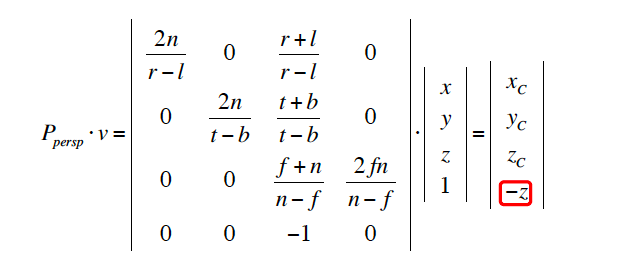
\includegraphics[width=.5\linewidth]{fourthcomp} 
%\end{figure}
Textures are images that are mapped over triangles on screen. However there are some issues that occur during mapping :
\begin{itemize}
\item UV coordinates are \textbf{floating point} numbers , while \textbf{texels} are indexed by integer numbers
\item The pixel shape on screen might correspond to several texels on the texture ( shape mismatch) 
\begin{figure}[H]
 \centering
 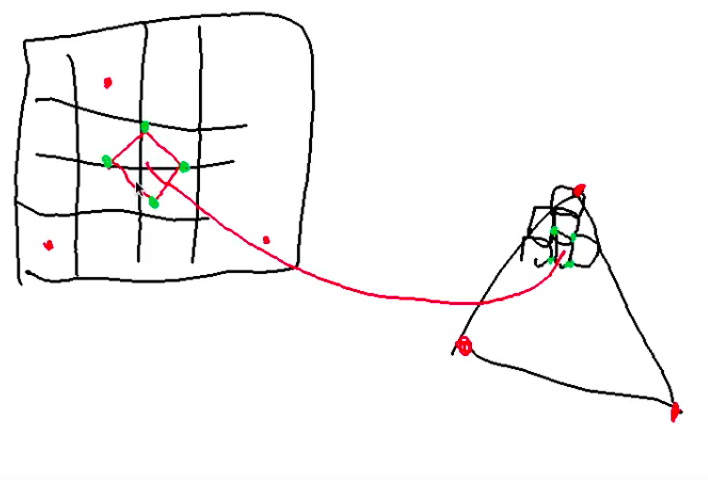
\includegraphics[width=.5\linewidth]{uvmissmatch} 
 \end{figure}
 When the texel is \textbf{larger} than the corresponding pixel a \textbf{magnification filtering} problem occurs. Vice-versa if the pixel corresponds to \textbf{several} texels a \textbf{minification filtering} problem occurs.
 \begin{figure}[H]
 \centering
 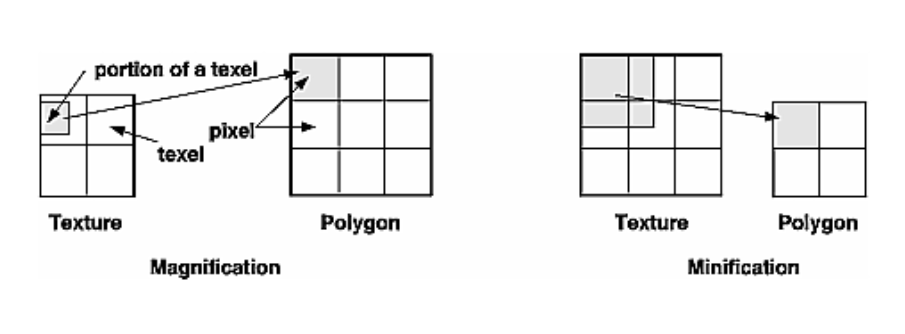
\includegraphics[width=.5\linewidth]{minimag} 
 \end{figure}
 Minification is the \textbf{tougher} of the two filtering problems : it requires fusing together pixels which can be very tricky as you can easily loose detail ( for example if the texture has a text on it the letters could become unrecognisable ) . 
\end{itemize}
The two filter problems can be solved also taking care of the floating to integer conversion.

\subsection{Magnification Filtering}
Two magnification filter are usually defined 
\begin{itemize}
\item \textbf{Nearest pixel}
\item \textbf{(bi)linear interpolation}
\end{itemize}
A texture of size $wxh$ is considered. Texels over :
\begin{itemize}
\item u-axis $\rightarrow$ indexed from $0 - (w-1)$
\item v-axis $\rightarrow$ indexed from $0 - (h-1)$
\end{itemize}
So texel $P[0][0]$ is on the bottom left:
\begin{figure}[H]
 \centering
 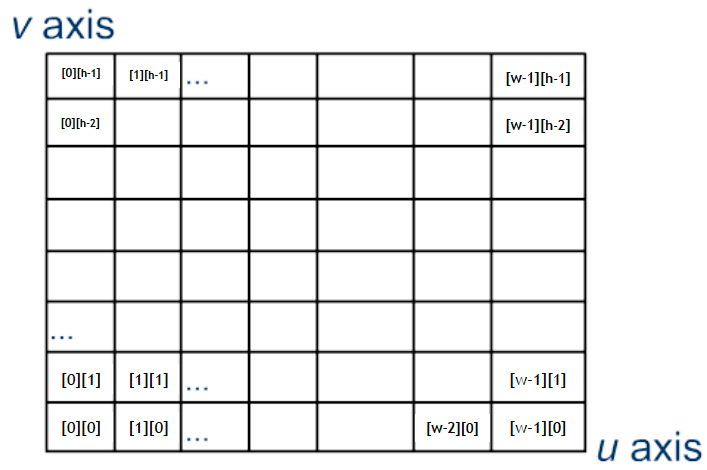
\includegraphics[width=.5\linewidth]{texturelayout} 
 \end{figure}

\subsubsection{Nearest Pixel}
With this technique the look-up procedure :
\begin{enumerate}
\item Transform the UV coordinates wrt the texture size : $$ x= u \cdot w $$ $$y = v \cdot h $$ where x,y are still \textbf{floating point} numbers ( as x,y $ \in [0,1]$ and w $\in [0,w-1]$ ,h $\in [0,h-1]$
\item Return the texel $p[i][j]$ that consider only the \textbf{integer part} of the scaled coordinates
$$ i = \lfloor x \rfloor $$
$$ j = \lfloor y \rfloor $$ 
\end{enumerate}
It is very fast and requires reading \textbf{one texel per pixel} but results in \textbf{blocky} images : this because close u-coordinates for example $ u_1 = .01 ,u_2 = .02 ...$ are multiplied by the width , for example 32 resulting in $x_1= .32 x_2 = .64 ...$ which results in $i_1= 0 ,i_2 = 0 ,i_3=0$.

\subsubsection{(Bi)Linear Interpolation}
Linear interpolation interpolates the color of the pixel from the values of its closest neighbours.
\begin{figure}[H]
 \centering
 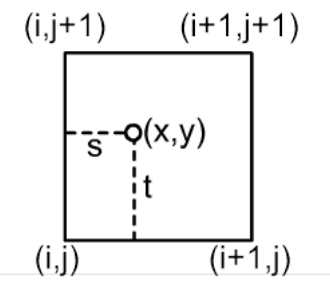
\includegraphics[width=.5\linewidth]{bilinear} 
 \end{figure}

\begin{enumerate}
\item  $$ x= u \cdot w$$ $$ y= v \cdot h$$
\item $$ i = \lfloor x - 0.5 \rfloor $$
$$ j = \lfloor y -0.5 \rfloor $$ 
This is done because the pure color is considered at the \textbf{center } of each texel
\item $$ s=x-i-0.5$$ $$ t = y-j-0.5$$
\end{enumerate}
\[
\boxed{p' = (1-t)[(1-s)p_{i,j} + s \cdot p_{i+1,j}]+t[(1-s)p_{i,j+1}+ s \cdot p_{i+1,j+1}]}
\]
The techniques is much \textbf{smoother} but requires \textbf{4 texture access} and \textbf{3 interpolations} per pixel. In the 1D case it requires 2 texels , 1 interpolation and in the 3D case it requires 8 texels and 7 interpolations.

\subsection{Minification Filtering}
Also minification can use \textbf{nearest pixel} and \textbf{linear interpolation} but with poor results as they both try to simply guess an intermediate value rather than averaging the texels that fall inside a pixel.
A good alternative is the \textbf{MIP-Mapping} technique.

\subsubsection{MultiploInParving-Mapping}
This techniques precomputes a set of scaled versions of the texture each one \textbf{halved in size} by averaging the values of the pixels and fetches the pixel from the one that is \textbf{closest} to the on-screen pixel size. A MIP-Map requires \textbf{$33\%$} extra space.

\begin{figure}[H]
 \centering
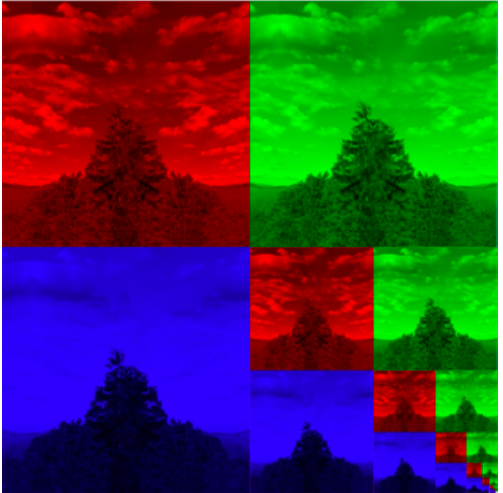
\includegraphics[width=.5\linewidth]{mipmap} 
\end{figure}
The pixel of the chosen image can be then \textbf{interpolated} or chosen with \textbf{nearest pixel} approach.

\subsection{UV Intervals}
Sometimes the u,v values can fall \textbf{outside} the $[0,1]$ range. Several behaviours and several alternatives are possible,with the main 4 being :
\begin{itemize}
\item \textbf{Clamp}
\item \textbf{Repeat}
\item \textbf{Mirror}
\item \textbf{Constant}
\end{itemize}
These techniques are applied at the \textbf{texel level} , so first the i,j indexes of the texels have to be computed ( already seen ) 

\subsubsection{Clamp}
Extends the colors of the border to the texels that are outside the $[0,1]$ range.
\begin{figure}[H]
 \centering
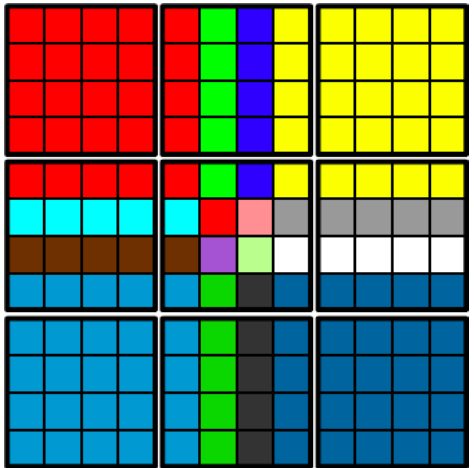
\includegraphics[width=.4\linewidth]{clamp} 
\end{figure}
Focusing on coordinate u , i is the index of the texel required by nearest pixel or linear interpolation. The value of the index of the texel fetched  from the texture can be determined as : 
\[ i_{Act} =
\begin{cases}
	0 & i < 0\\
	i & 0 \leq i < w \\
	w-1 & i \geq w
\end{cases}
\]
Same goes for v and index j :
\[ j_{Act} =
\begin{cases}
	0 & j < 0\\
	i & 0 \leq j < h \\
	h-1 & j \geq h
\end{cases}
\]

\subsubsection{Repeat}
The repeat strategy repeats the pattern indefinitely many times both in the horizontal and vertical direction. It can be computed as : 
$$ i_{Act} = mod(i,w) $$
$$ j_{Act} = mod(j,h)$$
where $$ mod(i,w) $$ is a \textbf{non-negative integer less than w} such that exists an integer k : 
$$ k \in Z \quad, 0 \leq mod(i,w) < w ,\quad k \cdot w+mod(i,w)=i$$
\begin{figure}[H]
 \centering
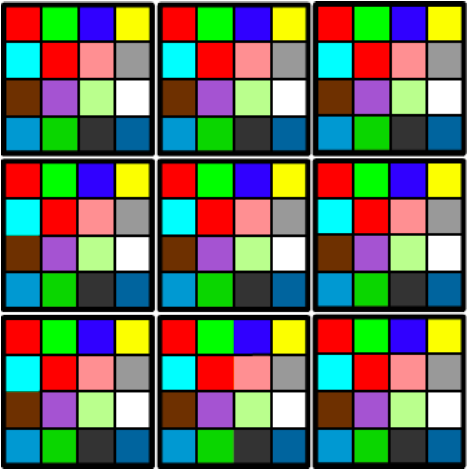
\includegraphics[width=.4\linewidth]{repeat} 
\end{figure}

\subsubsection{Mirror}
Similar to repeat but at each replication it flips the texture.
$$ i_{Tmp} = mod(i,2w) \quad \{ 0 \leq i_{Tmp} \leq 2w \}$$
\[ i_{Act} =
\begin{cases}
	i_{Tmp} & i_{Tmp} < w\\
	2w-i_{Tmp}-1 & i_{Tmp} \geq w \\
\end{cases}
\]
The second case is when the texel should be flipped.
\begin{figure}[H]
 \centering
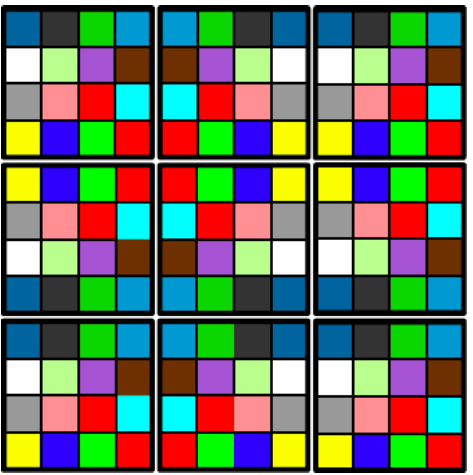
\includegraphics[width=.4\linewidth]{mirror} 
\end{figure}

\subsubsection{Constant}
The constant behaviour replaces the sample of the texture that fall outside the $[0,1]$ range with a default color $c_d$ :
\[ c =
\begin{cases}
	c_d & i < 0\\
	c[i] & 0 \leq i < w \\
	c_d & i \geq w
\end{cases}
\]
\begin{figure}[H]
 \centering
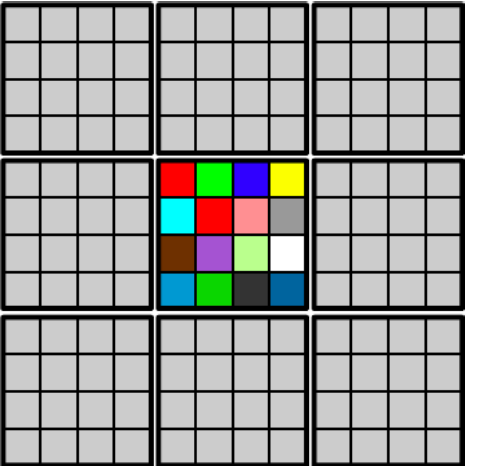
\includegraphics[width=.4\linewidth]{constant} 
\end{figure}
This is the \textbf{only technique} that return the texel \textbf{color} instead of the position.